%!TEX root = ../DSGEnotes.tex
\chapter{似然估计}
\label{sec:mle-model}

\section{线性模型}
\label{sec:linear-model}

设一组含有$n$个观察数据的随机变量$\left\{ y_{i} \right\}, \, i = 1,\ldots,n$。假定其中每个观察符合正态分布$y_{i} \sim \mathcal{N} \left( \mu_{i}, \sigma^{2} \right)$。由设定可见,对于$i,j \in [1,n], \, i \neq j$,均值也许不同,但方差相同。

正态分布(normal distribution)\index{normal distribution! \dotfill 正态分布}又称高斯分布(Gaussian distribution)\index{Gaussian distribution \dotfill 高斯分布},如$y_{i}$的概率密度方程(probability density function, PDF)\index{probability density function (PDF) \dotfill 概率密度方程} $f\left( y_{i} \right)$定义为
\begin{equation}
  \label{eq:mle-pdf-def}
  f \left( y_{i} \right) = \frac{1}{\sqrt{2 \pi \sigma^{2}}}
  \exp \left[
  - \frac{1}{2} \frac{
  \left( y_{i} - \mu_{i} \right)^{2}
  }{
  \sigma^{2}
  }
   \right],
\end{equation}
均值为$0$方差为$1$的高斯分布,见图\ref{fig:mle-pdf}所示。

\begin{lstlisting}[language=R]
# 正态分布的概率密度方程(均值=0,方差=1)
x <- seq(-4,4,length=100)
hx <- dnorm(x)
plot(hx ~ x, type="l", lty = 1, col="blue",
     xlab="y", ylab="Density",
     main = "Probability Density Function (normal distribution)")
\end{lstlisting}

\begin{figure}[htbp]
  \caption{正态分布的概率密度方程}
  \centering
  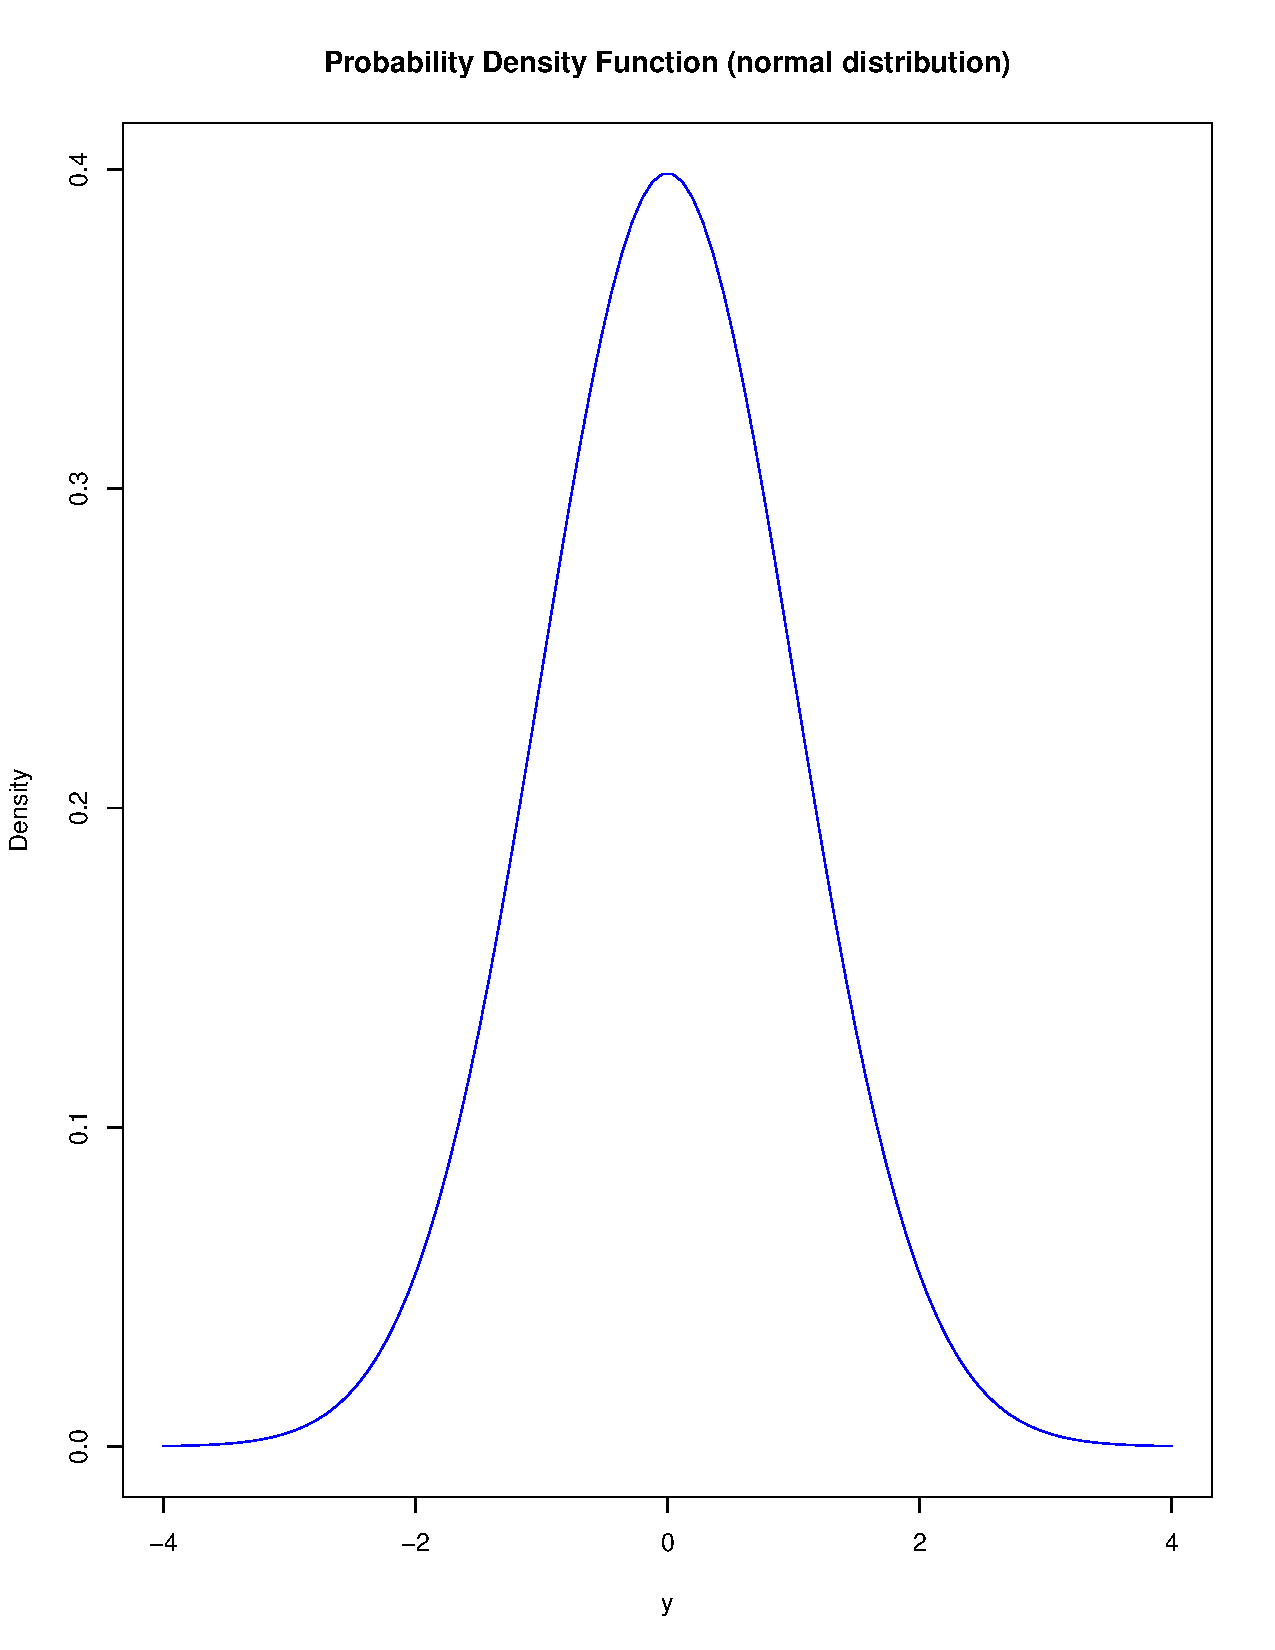
\includegraphics[width=8cm]{./Figures/20180421-pdf-function}
  \label{fig:mle-pdf}
%
%  \small{Source: PBOC.}
\end{figure}

现在引入额外的假定,对于全部$i, j \in [0,n], \, i \neq j$,设观测数据$y_{i}$和$y_{j}$相互独(mutually independent),即$\cov \left( y_{i}, y_{j} \right) = 0$。这使得我们能够计算观测数据集中全部数据的联合分布(joint distribution),即$\prod_{i=1}^{n} f \left( y_{i} \right)$,进而勾勒出似然方程,用于进一步的估计和检测。

把$\left\{y_{i}\right\}_{i=1}^{n}$表示为一个$(n \times 1)$的列向量$Y$,对应均值$E Y = \mu$,方差协方差矩阵$\var(Y) = \sigma^{2} I$,其中$I$是单位矩阵。列向量$\mu = \left\{ \mu_{i} \right\}_{i=1}^{n}$。
由于$n$个观测变量$y_{i}$彼此不相关且方差相同,$\var(Y)$满足以下特征:对角元素全是$\sigma^{2}$,非对角元素全是$0$。进而$Y$呈多元正态分布(multivariate normal distribution)\index{normal distribution!multivariate \dotfill 多元正态分布}
\begin{equation}
  \label{eq:multivariate-normal-distribution}
  Y \sim \mathcal{N}_{n} \left( \mu, \sigma^{2} I \right).
\end{equation}

来看\eqref{eq:multivariate-normal-distribution}的模型。假定$Y = y_{1}, y_{2}, \ldots, y_{n}$与某组预测变量$X = x_{1}, x_{2}, \ldots, x_{n}$有关,进一步说,第$i$个观测变量$y_{i}$的期望值$\mu_{i}$,与$x_{i1}, x_{i2}, \ldots, x_{ip}$有关,呈线性关系,满足
\begin{equation}
  \label{eq:mle-linear-relationship-yx-np}
  \mu_{i} = \beta_{1} x_{i1} + \beta_{2} x_{i2} + \ldots + \beta_{p} x_{ip} \Longleftrightarrow \mu_{i} = x_{i}^{\top} \beta,
\end{equation}
其中$x_{i}^{\top}$是由$p$个预测变量$x_{i1}, x_{i2}, \ldots ,x_{ip}$组成的行向量。待求解的未知系数$\beta = \beta_{1}, \ldots, \beta_{p}$称回归系数。将全部$n$个\eqref{eq:mle-linear-relationship-yx-np}加总可得
\begin{equation}
  \label{eq:mle-linear-relationship-mu-x-beta}
  \underset{\left( n \times 1 \right)}{\mu} =
  \underset{\left( n \times p \right)}{X}
  \underset{\left( p \times 1 \right)}{\beta},
\end{equation}
我们常将解释变量的矩阵$X$称为模型矩阵(model matrix)\index{model matrix \dotfill 模型矩阵}或设计矩阵(design matrix)\index{design matrix \dotfill 设计矩阵}。对应地,$X \beta$称线性预测子(linear predictor)。

最简单的线性模型可以假定每个观测数据的期望值都相同$\mu_{i} = \mu \, \forall \, i$,称零模型(null model)\index{null model \dotfill 零模型}。另一个极端是$\mu_{i} \neq \mu_{j} \, \forall \, i \neq j$,称饱和模型(saturated model)\index{saturated model \dotfill 饱和模型},此时观测数据量$n$越大,待估计的线性系数$\beta$数量就越多($p \times n$)。

零模型和饱和模型是两个极端。现实应用中常取折中,致力于分析导致线性预测子$X \beta$产生结构差异的系统性原因,进而分析观测数据$y$和均值$\mu$之间的非结构性差异(或称随机差异),用误差项来表示。

\section{参数估计}
\label{sec:mle-parameter-estimation}
来看模型$\mu_{i} = x_{i}^{\top} \beta$。问题:如何估计参数$\beta, \sigma^{2}$?

\subsection{回归系数的估计}
\label{sec:mle-estimation-beta}
我们的求解思路是,建立似然方程(likelihood function, LHF)\index{likelihood function (LHF)\dotfill 似然方程},选取使(对数)似然方程最大化的参数值。如果观测数据之间互相独立,那么LHF是一组正态PDF \eqref{eq:mle-pdf-def}的乘积
\begin{equation}
  \label{eq:mle-lhf-pdf-product}
  \log L \left( \beta, \sigma^{2} \right) = - \frac{n}{2} \log \left( 2 \pi \sigma^{2} \right) - \frac{1}{2} \sum_{i=1}^{n}
  \frac{
  \left( y_{i} - \mu_{i} \right)
  }{
  \sigma^{2}
  },
\end{equation}
$\mu_{i}$如\eqref{eq:mle-linear-relationship-yx-np}所定义。RHS中可定义残差平方和(residual sum of squares, RSS)\index{residual sum of squares (RSS) \dotfill 残差平方和}
\begin{equation}
  \label{eq:mle-rss-def}
  RSS (\beta) = \sum_{i=1}^{n} \left( y_{i} - \mu_{i} \right)^{2}
  = \left( y - X \beta \right)^{\top} \left( y - X \beta \right).
\end{equation}

不难看出,在给定$\sigma^{2}$值不变的情况下,最佳系数$\hat{\beta}$的选取符合
\begin{equation}
  \label{eq:mle-lhf-argmax-beta}
  \hat{\beta} =\underset{\beta}{\argmax} \log L \left( \beta, \sigma^{2} \right)
  = \underset{\beta}{\argmin} \frac{\rss(\beta)}{\sigma^{2}},
\end{equation}
也即,我们的目标是选取合适的$\beta = \hat{\beta}$,使对应的模拟值$\mu_{i}$尽可能接近实际观测值$y_{i}$。

求解$\argmin \rss (\beta)$等价于求解$\rss \left( \hat{\beta} \right) =0$,即
\begin{equation*}
  y - X \hat{\beta} = 0 \quad \Rightarrow y = X \hat{\beta} \quad \Rightarrow X^{\top} y = X^{\top} X \hat{\beta}
\end{equation*}
如果模型矩阵$X$列满秩,那么$X^{\top} X$也是满秩的,因而$X^{\top} X$可逆。由此可得线性系数$\hat{\beta}$的OLS估计式(同时也是MLE估计式)
\begin{equation}
  \label{eq:mle-argmin-beta-hat-estimation}
  \hat{\beta} = \left( X^{\top} X \right) X^{\top} y.
\end{equation}
我们将这个方程称为正规方程(normal equation)\index{normal equation \dotfill 正规方程}。

反之,如果$X$不是列满秩的,可以计算$\left( X^{\top} X \right)^{\dagger}$,称为伪逆矩阵(第\ref{sec:simple-pseudo}节)。但比起这种相对复杂的计算来,还是直接删除$X$中的冗余列更加方便。当前大多数主流统计软件都足够只能,可以自动识别并删除冗余列。

求解正规方程\eqref{eq:mle-argmin-beta-hat-estimation}需要借助数值方法。数值方法有多种,常见的如
\begin{itemize}
  \item 从$\left( X^{\top} X \right)$入手,方法如高斯消元法(第\ref{sec:numlin-gaussian-elimination}节)、Cholesky分解(第\ref{sec:numlin-factorization-cholesky}节)等。
  \item 对模型矩阵$X$做因子分解,如
  \begin{itemize}
    \item Householder reflections
    \item Givens rotations
    \item Gram-Schmidt正交(第\ref{sec:orthogonality-polynomials}节),等
  \end{itemize}
\end{itemize}
结合大多数主流数值计算软件,可以执行上述数值运算。

基于\eqref{eq:mle-lhf-argmax-beta},利用最小化RSS方法测得的系数$\hat{\beta}$,是一个不依赖于$\sigma^{2}$的值——方差值是事先给定的。因此我们称$\hat{\beta}$为最大似然法的全局最大解(global maximum)。

对于零模型的情况:$X$是一组$1$构成的向量;$\left( X^{\top} X \right) = n$和$X^{\top} y = \sum_{i=1}^{n} y_{i}$是两个标量;$\hat{\beta} = \bar{y}$是样本的均值。这就是说,计算出的样本均值,可堪称是在线性模型中做最大似然估计的一个最简单的例子。

关于MLE $\hat{\beta}$,有以下几个有趣的性质。

\begin{enumerate}
\item BLUE
\begin{enumerate}
  \item 如果模型设定正确,即从(弱的)意义上说,给定$x_{i}$的情况下,观测$y_{i}$的期望值$\mu_{i}$就等于$x_{i}^{\top} \beta$,此时的OLS估计$\hat{\beta}$是个无偏估计(unbiased estimator),OLS 估计$\hat{\beta}$的期望值就等于真实参数值$\beta$
\begin{equation}
  \label{eq:mle-hat-beta-unbiased}
  E \hat{\beta} = \beta.
\end{equation}
  \item 如果观测数据之间彼此不相关$\cov \left(y_{i}, y_{j} \right) = 0, \, \forall \, i \neq j$,并且同方差$\sigma_{i}^{2} = \sigma_{j}^{2}= \sigma^{2}$。那么,一方面根据\eqref{eq:mle-rss-def}-\eqref{eq:mle-lhf-argmax-beta},$\hat{\beta}$是一个关于$y$的线性方程,另一方面根据假定,观测数据集合$Y$的方差协方差矩阵$\var(Y) = \sigma^{2} I$,那么OLS估计$\hat{\beta}$的方差协方差矩阵为
  \begin{equation}
    \label{eq:mle-hat-beta-varcov}
    \var \left( \hat{\beta} \right) = \left( X^{\top} X \right)^{-1} \sigma^{2},
  \end{equation}
  因此,基于观测数据,构建线性方程模型所做的全部无偏OLS估计$\left\{\beta\right\}$中,MLE估计$\hat{\beta}$是最佳线性无偏估计(best linear unbiased estimator, BLUE)\index{best linear unbiased estimator (BLUE) \dotfill 最佳线性无偏估计}。对于某一给定的观测样本,由于再没有其他无偏估计的方差会低于$\var \left( \hat{\beta} \right)$,我们称OLS估计$\hat{\beta}$是有效估计(efficient estomator)\index{efficient estimator \dotfill 有效估计}。
\end{enumerate}

\item OLS估计$\hat{\beta}$在大样本观测集合中的抽样分布,接近于多元正态分布,其均值和方差如\eqref{eq:multivariate-normal-distribution}所定义,满足
\begin{equation*}
  \hat{\beta} \sim \mathcal{N}_{p} \left( \beta, \left(X^{\top}, X \right)^{-1} \sigma^{2} \right).
\end{equation*}

\item 将前两个性质代入零模型,可见样本均值$\bar{y}$是对$\mu$的无偏估计;$\bar{y}$的方差为$\frac{\sigma^{2}}{n}$,在大样本下近似正态分布。

\item 前三条性质的生成,依赖于对观测数据的均值、方差协方差的最高到二阶矩条件的假设,包括
\begin{equation*}
  E Y = X \beta, \quad \var \left( Y \right) = \sigma^{2} I.
\end{equation*}

\item 基于观测数据的联合正态分布假定,所测得的OLS估计$\hat{\beta}$也是MLE。如果$Y \sim \mathcal{N}_{p} \left( X \beta, \sigma^{2} I \right)$,那么$\hat{\beta}$的样本分布恰好也是多元正态分布,对应的、方差也是
\begin{equation*}
  \hat{\beta} \sim \mathcal{N}_{p} \left( \beta, \left(X^{\top}, X \right)^{-1} \sigma^{2} \right).
\end{equation*}.
\end{enumerate}

需要指出的是,上属性质虽然重要,但不应被过分夸大:只有在小样本数据的统计推断中,才需要假定观测数据是正态分布的。而真正重要的假设其实是观测数据之间彼此不相关,同方差:这些对于大样本数据下的统计推断至关重要。

\subsection{方差的估计}
\label{sec:mle-estimation-variance}
将求得的OLS估计$\hat{\beta}$ \eqref{eq:mle-argmin-beta-hat-estimation}代回log LHF \eqref{eq:mle-lhf-pdf-product},可得一个关于方差$\sigma^{2}$的最大(对数)似然方程,又称描述似然方程(profile likelihood function)\index{profile likelihood function \dotfill 描述似然方程}
\begin{equation}
  \label{eq:mle-estimation-variance-plhe}
  \log L \left( \sigma^{2} \right)
  = - \frac{n}{2} \log \left( 2 \pi \sigma^{2} \right)
  - \frac{1}{2} \frac{
  \rss \left( \hat{\beta} \right)
  }{\sigma^{2}}.
\end{equation}

类似地,$\hat{\sigma}^{2} = \underset{\sigma^{2}}{\argmin} \partial \log L \left( \sigma^{2} \right)$,等价于求解$\underset{\sigma^{2}}{\arg} \left[ \frac{\partial \log L \left( \sigma^{2} \right)}{\partial \sigma^{2}} = 0 \right]$,求得的值为方差的MLE
\begin{equation*}
  \hat{\sigma}^{2} = \frac{\rss \left( \hat{\beta} \right)}{n},
\end{equation*}
需要指出的是,$\hat{\sigma}^{2}$是有偏估计;我们可以将分母用$n-p$代替$n$来变为无偏估计(类似于在估计方差时用$n0-1$代替$n$)。

在零模型中,方差$\sigma^{2}$的估计是样本方差:这是由于$\hat{\beta} = \bar{y}, \, \rss = \sum_{i=1}^{n} \left( y_{i} - \bar{y} \right)$。在正态分布的假定条件下,比值$\left( \frac{\rss }{\sigma^{2}}\right)$呈$\chi^{2}$分布(DoF n-p),并且与线性系数估计值$\hat{\beta}$无关。

小提示:使用$\chi^{2}$分布作为LHF来估计$\sigma^{2}$,比起使用高斯分步来同时估计$\beta, \sigma^{2}$来,会得到无偏估计。

\section{假设检验}
\label{sec:mle-hypothesis-testing}
如何对回归系数向量估计$\hat{\beta}$作假设检验?具体来说,这个问题可以分为两种情况
\begin{itemize}
  \item 对向量$\beta$中的某个系数$\beta_{i}$作显著程度检验,
  \item 对几个、甚至全部系数作显著程度检验,
\end{itemize}
本节介绍一些常见的检测方法,尤其是
\begin{itemize}
  \item 基于MLE的抽样分布的Wald检验,
  \item 似然率检验。
\end{itemize}

\subsection{Wald检验}
\label{sec:mle-wald-test}
